\documentclass[a4paper,14pt]{article}

%Font
\usepackage{fontspec}
\setmainfont{CMU Serif}[Ligatures=TeX]
\usepackage{polyglossia}
\setdefaultlanguage{russian}
\setotherlanguages{english}
\usepackage{emoji}
\setemojifont{TwemojiMozilla}

\usepackage{bookmark}
\usepackage{booktabs}
\usepackage{amsfonts}
\usepackage{amsmath}
\usepackage{amssymb}
\usepackage{amsthm}
\usepackage{array}
\usepackage{color}
\usepackage{xcolor}
\usepackage{calc}
\usepackage{longtable}
\usepackage{ragged2e}
\usepackage{extsizes}
\usepackage{hyperref}
\usepackage{ulem}
\usepackage{graphicx}
\usepackage{subfiles}
\usepackage{mdframed}
\usepackage{enumitem}

%Indents
\setlength{\parindent}{1.8em}
\setlength{\parskip}{0.5em}
\addtolength{\voffset}{-3cm}
\addtolength{\hoffset}{-2cm}
\addtolength{\textheight}{+6cm}
\addtolength{\textwidth}{+4cm}
%Element indents
\makeatletter
\newcommand{\mathleft}{\@fleqntrue\@mathmargin}
\newcommand{\mathcenter}{\@fleqnfalse}
\makeatother
\setlist{itemsep=0, topsep=0, partopsep=0}

%Tables
\renewcommand{\arraystretch}{1.2}
\setlength\LTpre{0}
\setlength\LTpost{0}

%Partition
\setcounter{secnumdepth}{1}
\makeatletter
\@addtoreset{section}{part}
\makeatother

%Theorems
\mdfdefinestyle{basic}{
    linewidth=1,
    outertopmargin = 0,
    outerbottommargin = 0,
%    innerrightmargin = 1cm,
}
\theoremstyle{definition}
\newtheorem{_key_}{Ключевые термины}[section]
\newtheorem{_theorem_}{Теорема}[section]
\newtheorem{_lemma_}[theorem]{Лемма}
\newenvironment{terms}{
    \begin{mdframed}[style=basic]
        \begin{Center}
            \textbf{\large Термины}
        \end{Center}
        \begin{description}[style=nextline, itemsep=0.2em, partopsep=0, topsep=0]
            \mathleft}
            {
        \end{description}
    \end{mdframed}\par}


\title{Математическая статистика}
\author{Даня Дудаф}
\date{20 августа 2021 г.}

\begin{document}
    %Equation indents
    \abovedisplayshortskip=-0.9em
    \abovedisplayskip=0.1em
    \belowdisplayskip=0em

    %Header info
    \maketitle
    \thispagestyle{empty}
    \tableofcontents
    \newpage

    \section{Разведочный анализ данных}

\subsection{Типы данных}
\begin{terms}
    \item[Непрерывные данные] Любое значение в интервале.
    \item[Дискретные данные] Целочисленные значения.
    \item[Категориальные данные] Из определенного набора значений.
    \item[Двоичные данные] Истина/ложь.
    \item[Порядковые данные] Упорядоченные категориальные данные.
\end{terms}

\subsection{Фреймы данных}
\begin{terms}
    \item[Data frame] Таблица данных.
    \item[Признак (feature, атрибут, предиктор, параметр, переменная)] Столбец в таблице.
    \item[Исход (outcome, отклик)] Предсказываемый столбец таблицы.
    \item[Записи] Строка в таблице.
\end{terms}

\subsection{Оценки центрального значения}
\begin{terms}
    \item[Среднее]
    \begin{equation*}
        \overline{x} = \frac{\sum_{n}^{i} x_i}{n}, \quad
        \text{$x_i$ - значение данных.}
    \end{equation*}
    \item[Среднее усеченное]
    \begin{equation*}
        \overline{x} = \frac{\sum_{n-z}^{i=z+1} x_i}{n - 2z}, \quad
    \text{с пропуском $z$ самых малых и самых больших значений.}
    \end{equation*}
    \item[Среднее взвешенное]
    \begin{equation*}
        \overline{x}_w = \frac{\sum_{n}^{i} w_i x_i}{\sum_{n}^{i} w_i}, \quad
        \text{$w_i$ - вес данных.}
    \end{equation*}
    \item[Медиана] Значение, при котором половина сортированных данных находится
    выше и ниже данного значения.
    \item[Медиана взвешенная] Значение, при котором половина суммы весов находится
    выше и ниже данного значения.
    \\\hline
    \item[Выброс (outlier)] Сильно отличающееся от большинства значение данных.
    \item[Robust] Устойчивый к выбросам.
\end{terms}
Среднее - неробастный метрический показатель, остальные метрики более устойчивые к выбросам.

\subsection{Оценки вариабельности}
\begin{terms}
    \item[Отклонение (ошибка)] $\overline{x} - x_i$
    \item[Размах] $|max(X) - min(X)|$
    \item[Дисперсия]
    Мера разброса значений случайной величины относительно её математического ожидания.
    \begin{equation*}
        D(X) = \frac{\sum_{i=1}^n (x_i - \overline{x})^2}{n - 1}
    \end{equation*}
    \item[Стандартное отклонение]
    $\sigma(X) = \sqrt{D(X)}$
    \item[Среднее абсолютное отклонение]
    \begin{equation*}
        S_a(X) = \frac{\sum_{i=1}^n |x_i - \overline{x}|}{n}
    \end{equation*}
    \item[Медианное абсолютное отклонение от медианы]
    Медиана$(|x_1-m|, |x_2-m|, \ldots, |x_N-m|)$, $m$ - медиана.
    \item[Процентиль] P процентов принимает значение меньше этого.
    \item[Межквартильный размах] Разность между 75-м и 25-м процентилем.
    \\\hline
    \item[Порядковые статистики] Статистические показатели на основе сортированных данных.
\end{terms}
Дисперсия и стандартное отклонение чувствительны к выбросам.
\par \textbf{Визуализация распределения данных:}
\begin{itemize}
    \item Гистограмма / Частотная таблица
    \item Коробчатая диаграмма
    \item График плотности
\end{itemize}

\subsection{Оценка двоичных и категориальных данных}
\begin{terms}
    \item[Мода] Наиболее часто встречающееся значение или категория.
    \item[Математическое ожидание]
    \begin{equation*}
        E(X) = \sum_{n}^{i} p_i x_i, \quad
        \text{$p_i$ - вероятность наступления исхода.}
    \end{equation*}
\end{terms}
\textbf{Визуализация категориальных данных:}
\begin{itemize}
    \item Столбчатая диаграмма
    \item Круговая диаграмма
\end{itemize}

\subsection{Зависимость двух переменных}
\begin{terms}
    \item[Коэффициент корреляции (Пирсона)] Метрический показатель, который измеряет степень,
    с какой числовые переменные связаны друг с другом (от $-1$ до $1$).
    \begin{equation*}
        r(X, Y) = \frac{\sum_{i=1}^{n} (x_i - \overline{x}) (y_i - \overline{y})}{(n - 1) \sigma(x) \sigma(y)}
    \end{equation*}
    \item[Корреляционная матрица] Таблица, в которой строки и столбцы --- это переменные, и значения ячеек ---
    корреляции между этими переменными.
\end{terms}
Коэффициент корреляции Пирсона не является робастным показателем.
\par \textbf{Визуализация корреляции:}
\begin{itemize}
    \item Диаграмма рассеяния
\end{itemize}

\subsection{Многомерный анализ}
\begin{terms}
    \item[Таблицы сопряженности (contigency tables)] Сводка количеств нескольких категориальных переменных.
\end{terms}
\textbf{Визуализация зависимости нескольких переменных:}
\begin{itemize}
    \item График с шестиугольной сеткой (hexagonal binning)
    \item Тепловая карта
    \item Контурный график
    \item Скрипичный график (violin plots)
\end{itemize}

    \section{Распределения данных}

\subsection{Отбор данных}
\begin{terms}
    \item[Генеральная совокупность (population)] Полный наблюдаемый набор данных.
    \item[Выборка (sample)] Подмножество набора данных.
    \item[Репрезентативная выборка] Достоверно представляет всю популяцию в целом.
    \item[Смещение (bias)] Систематическая ошибка отбора.
    \item[Смещенная выборка] Представляющая популяцию в искаженному виде.
    \item[Случайный отбор] При котором каждый элемент имеет одинаковую вероятность попасть в выборку.
    \item[Простая случайная выборка] Результат случайного отбора.
    \item[Страты] Множество элементов с некоторым схожим признаком.
    \item[Стратифицированный отбор]
    Разделение генеральной совокупности на страты и случайный отбор элементов из каждой страты.
\end{terms}
Случайный отбор может производиться как с возвратом элементов, так и без него.
\par Качество данных часто имеет большее значение, чем их количество.

\subsection{Выборочное распределение статистики}
\begin{terms}
    \item[Выборочная статистика] Метрический показатель для выборки.
    \item[Распределение данных] Частотное распределение значений в наборе данных.
    \item[Выборочное распределение] Частотное распределение выборочной статистики на выборках.
    \item[Центральная предельная теорема] Тенденция выборочного распределения принимать нормальную форму
    по мере увеличения размера выборок.
    \item[Стандартная ошибка] Изменчивость выборочной статистики на выборках.\\
    $\sigma / \sqrt{n}$, \quad \sigma --- стандартное отклонение.
\end{terms}

\subsection{Бутстрап}
\begin{terms}
    \item[Бутстрап] Взятие выборки с возвратом из популяции.
    \item[Повторный отбор (resampling)] Бутстрап с перестановками.
\end{terms}
\textbf{Применения бутстрапа:}
\begin{itemize}
    \item Определение вариабельности выборочной статистики.
    \item Работа с выборками без использования математических приближений.
    \item Оценка выборочных распределений для статистик.
    \item Бэггинг (Bootstrap aggregating): агрегирование предсказаний.
    \item Создание доверительных интервалов.
\end{itemize}

\subsection{Доверительные интервалы}
\begin{terms}
    \item[Доверительный интервал] С заданной вероятностью накрывает оцениваемый параметр популяции.
    \item[Уровень значимости] Вероятность непопадания значения в доверительный интервал.
    \item[Уровень доверия] Вероятность покрытия интервалом значения.
\end{terms}

\subsection{Нормализация}
\begin{terms}
    \item[Нормализация] Преобразование данных к безразмерным единицам в рамках заданного диапазона
    или с заданным свойством.
    \item[Стандартизация] Преобразование исходного набора в новый с $\overline{x} = 0$ и $\sigma = 1$\\
    \begin{equation*}
        z = \frac{x - \overline{x}}{\sigma}
    \end{equation*}
    \item[Минимакс] Преобразование исходного набора в диапазон $[0, 1]$.
    \begin{equation*}
        x_{norm} = \frac{x - x_{min}}{x_{max} - x_{min}}
    \end{equation*}
\end{terms}
Ключевая цель нормализации --- приведение данных к единому виду,
который позволит сравнивать их между собой или использовать для расчёта схожести объектов.

\subsection{Распределения}
\begin{terms}
    \item[Квантиль-квантильный график (QQ-plot)] Показывает связь между наблюдаемыми значениями
    и стандартизированными квантилями. %TODO
    %TODO add info about distributions
\end{terms}
В нормальном распределении 68\% данных находятся в пределах одного
стандартного отклонения от среднего и 95\% — в двух стандартных отклонениях.\\
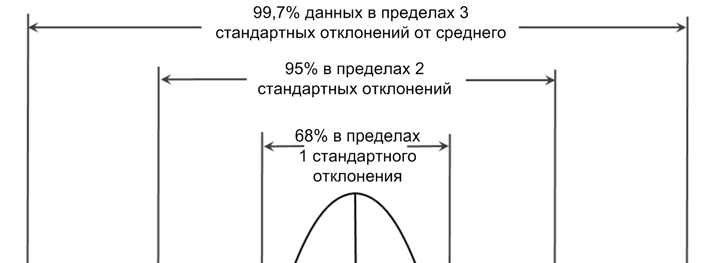
\includegraphics[scale=0.5]{50 notions/img/norm_dist1}\\
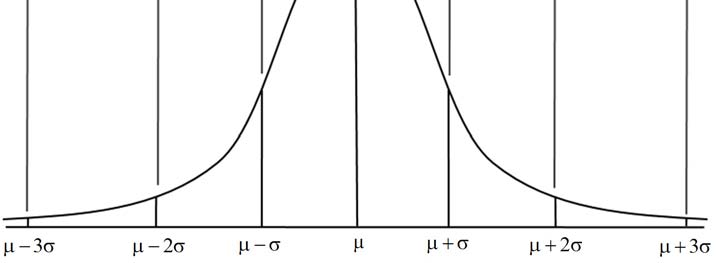
\includegraphics[scale=0.5]{50 notions/img/norm_dist2}

    %    \section*{Sources}
\label{sec:sources}
\addcontentsline{toc}{section}{\nameref{sec:sources}}

\begin{itemize}
    \item[] Fiona Davis and Wayne Rimmer --- Active grammar level 1 (2011);
    \item[] Fiona Davis and Wayne Rimmer --- Active grammar level 2 (2011);
\end{itemize}       %TODO standart resource list
\end{document}
